\chapter{Design}
\label{chap:design}

\section{Introduction}
\label{sec:designintroduction}

The goal of this thesis is to develop a modularized and production grade user simulator that can be re-targeted for new domains and provide a framework to produce training data and train dialog agents. The overall design for the simulator was inspired by the work done by \cite{li_usersim} and the formalization of hidden user agenda models by \cite{Schatzmann2009TheHA}. 

Underlying the simulator is a framework that consists the following components:
\begin{itemize}
	\item \textbf{User Simulator}: An agenda based user modeling component that generates natural language speech utterances to simulate what an actual human would say in the context of task-completion dialog activity. 
	\item \textbf{Dialog Agent API}: A set of methods to allow a researcher to provide an agent(s) that simulate how the system / dialog agent would respond 
	\item \textbf{Dialog Manager}: A coordinator component that tracks the current state of the dialog and facilitates the conversation between the user simulator and dialog agent/system. Add the end of the simulated conversation, the manager will evaluate and score the conversion. 
\end{itemize}

\section{User Simulator} 

The user simulator is responsible for imitating a real user and generating realistic speech utterances. Here we assume the user is an actor that is attempting complete task. For example, the user may want to travel to Japan and is attempting to book a flight there. That user could then interact with a travel agent chatbot in order to get assistance in identifying the appropriate flight and purchasing tickets. In order to model and represent a user, we will utilize the formalization of the hidden user agenda described in \cite{Schatzmann2009TheHA}.

 One of the primary assumptions here is that user has intentionally engaged with the dialog agent in order to complete their task. At the outset of the conversation, the user will have some specific goal in mind (order Indian food, book a flight to Japan, etc). The dialog agent will attempt to learn user's goal by asking the user a set of clarifying questions. Schatzmann and Young introduces the idea of a hidden user agenda as a mechanism to represent the sequence of dialog acts and utterances a user will say in the context of that conversation. At each step of a task-completion dialog, the user is either responding to the dialog agent or initiating a new conversation direction. The user agenda provides an efficient way and formal structure to represent the pending set of dialog acts the user will communicate to the dialog agent.
 
Socrates Simulator implements the Schatzmann and Young's concept of user agenda and user goal as first class objects. The conversion from the formal representation to code is rather straightforward as there are analogous data structures. We will defer discussing implementation details until the next chapter. The subsections below will further describe how the user goal and agenda is defined. 

\subsection{User Goals} 
The user goal captures explicitly both user's preferences and missing information needs they are trying to fill. For example, take a user who wants to find an Indian restaurant in Central square for dinner. We can decompose this goal into two distinct components. The first is the user's explicit preferences. In this example, their preferred cuisine is Indian. The second component is implicit and unknown to the user. They are looking for a restaurant or more specifically the name and presumably the restaurant's phone number and address. This information is unknown but can be broken down into discrete pieces of information the user will attempt to elicit from the dialog agent as a request for more information. 

Formally, Schatzmann and Young defines the user goal \textit{G} as \textit{G = (C,R)}, where \textit{C} consists of constraints or the user's explicit preferences and \textit{R} represents the user's requests. The constraints and requests are explicitly represented as slot-value pairs. \ref{fig:goals1} below shows how one could represent the goal of user looking for a bar. 

\begin{figure}[h!]
	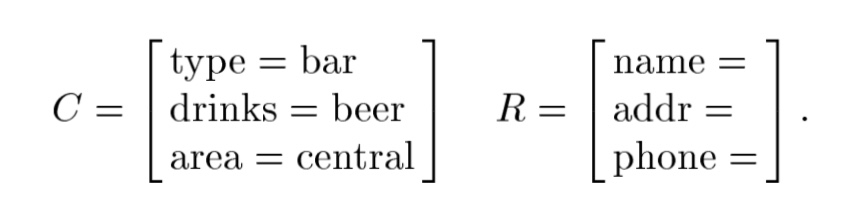
\includegraphics[width=\linewidth]{diagrams/schatzmann_goal_fig.jpeg}
	\caption{Example User goal. User wants the name, address and phone number of a cheap bar in central.  }
	\label{fig:goals1}
\end{figure}

The concept of a goal abstractly turns out to be useful in also driving the dialog manager's simulations. We abstract the idea of goal and make it available to both the user and dialog agent api as way to track the internal state of each speaker. 

\subsection{User Agenda} 

Schatzmann and Young define the user agenda as a “[stack] structure of pending dialogue acts [which] serve as a convenient mechanisms for encoding the dialogue history and user’s ‘state of mind’ ” \cite{Schatzmann2009TheHA}. Formally, at any time t, the user is in a state su  and takes an action au,which transitions into an intermediate state s’u. During this intermediate state, the user will receive an action from the system (machine) am, which will transition dialog to next state s’’u and the cycle will reset. The result is a sequence of alternating turns between the user and system (i.e. su -> au -> s’u -> am -> s’’u -> … ), which represents the conversation state over time t.
 
The user agenda A is stack-like structure which contains all pending user actions. User actions are actualized through popping the stack and the agenda is updated by pushing back onto the stack. A user act is a representation of the user’s intent, which will eventually be translated into a speech utterance. The stack may also contain other actions that will affect the user when popped. For example, the system can communicate a restaurant suggestion, which would fill the one of the request slots for restaurant name.  

At the start of the dialog a new goal is randomly generated from the provided dialog domain. An accompanying agenda is then generated to represent the potential sequential of events. 

\begin{figure}[h!]
	\caption{Example User Agenda }
	\label{fig:goals1}
\end{figure}


Below is an  example of the a sample user agenda that Schatzmann and Young provide in the context of a user asking the dialog system for a bar recommendation [6]. The states of the conversation are indexed by time t. Note, Schatzmann and Young use constraints C, which would be the equivalent of inform slots in our representation. In the first turn, the user simulator generates a set of constraints (bar serving beer in central) and goals (name, address, and phone for a bar that meets the constraints in C0). This set of inform and request slots are translated into a user action stored in A0. When the system initiates the conversation, the user simulator pops two inform actions which translate into the user utterance “I’m looking for a nice bar serving beer”. When the system at t=1, responds “Ok, a wine bar. What price range?” the agenda updated to include a new inform intent (inform(prange=cheap)). Also added is a negate action, as the user asked beer and not wine. 

Over the course of the conversation the agenda is updated, as are the request slots. The conversation ends at t=5, when bye() is popped and the agenda stack is empty. The conversation will then be evaluated based on how well the request slots were filled.



\section{Dialog Model}

\subsection{Overview}

Add paragraph here about high level design and how all component fit together. 

Give example of simple conversation flow.


\subsection{Design Philosophy}

At a high level, our aim is to develop a framework to allow dialog researchers to simulate a conversation between the user simulator and dialog agent. The framework needs to be modular so that it can be quickly adapted to support new dialog domains and experiments. Each major component of the framework is represented as a python class. Additionally, I promoted dialog actions, goals, and domain knowledge bases to first class objects, rather than implementing them at the lower dictionary level. As first class objects, I can standardize the communication, APIs, and management of these pieces and ensure more consistent behavior.

Additionally, we want to provide as much flexibility and freedom to the researcher and limit what is hard-coded. I follow the configuration first approach leveraged in the development of AllenNLP, a deep learning for NLP tool developed at the Allen Institute for Artificial Intelligence. The code is generalized and the user defines particular implementation details in configuration file. 

To support a configuration driven approach, each configurable module will have a use defined yaml or json file. For smaller configuration details, the user will prefer using yaml which is more human readable. 

The yaml format is simple and has a very low learning curve. It follows a basic key value pair paradigm, where keys have clear semantic meaning and values can be represented in a variety of data structures. 
\begin{figure}[h!]
	\caption{Example yaml section. }
	\label{fig:ex_yaml}
	\begin{lstlisting}
		# Dialog Simulation settings
		simulation_rounds: 10
		max_turns: 8
		first_speaker: usersim
		reward: 10
		simulation_output_path: data/simulated_dialogs/
		save_history: True
		save_location: "data/simulated_dialogs/"
		save_type: json
	\end{lstlisting}
\end{figure}

\section{ Simulation Framework Components}

All components are represented as python classes. The ensuing section further describe the component's function, design, and any salient implementation details. 

\subsection{Dialog Action}
The fundamental unit of transaction for the simulator is the dialog action. It is an explicit semantic representation of the speech utterance that is machine readable. The dialog action consist of three key properties: the dialog act, a set of explicit params, and corresponding unparsed speech utterance. 


 

\subsection{Goals}

\subsection{Dialog Status}


\subsection{Speaker}

The speaker represents an actor that has the ability to speak and comprehend speech utterances. In our framework, the both user simulator and the dialog agent are represented by the same base speaker class. Both actors conceptually are identical in terms of functional behavior, in that they both listen and comprehend speech utterances and in turn respond by speaking. As such, both the user simulator and dialog agent can be represented in the same way to the dialog manager. In fact, the entire conversation round can be expressed in two lines: 

\begin{figure}[h!]
	\caption{Psuedo code for conversation round.}
	\label{fig:conv_round}
	\begin{lstlisting}
	# Assuming user speaks first 
	# 1. User Simulator takes turn and speaks
	user_action = user_simulator.next(previous_agent_action, turn_number)
	# 2. Agent takes turn and responds to user 
	agent_action = agent.next(previous_user_action, turn_number)
	\end{lstlisting}
\end{figure}

The speaker class has four basic functions (\textit{next, reset, get utterance, and parse utterance}) and three properties (\textit{nlg model, nlu model, and dialog status}). When the speaker is initialized, the natural language object and the natural language understanding object are passed to the constructor. We abstract away the implementation of how the speaker speaks and parses speech in order maintain separation of concerns and also empower the researcher to be able to experiment with multiple techniques. 

The \textit{next} method is the primary driver how the speaker behaves. For the dialog agent class, the next method functions as an API to the simulator. It is assumed that the dialog agent will live and operate external the simulator. The researcher can define how the dialog agent will interact with the user simulator here. For the user simulator, the bulk of the logic will reside here. The \textit{get utterance} and \textit{parse utterances} methods are simply wrappers for the speaker's nlg and nlg objects. The primary parameter for next is the previous dialog action. 

\begin{figure}[h!]
	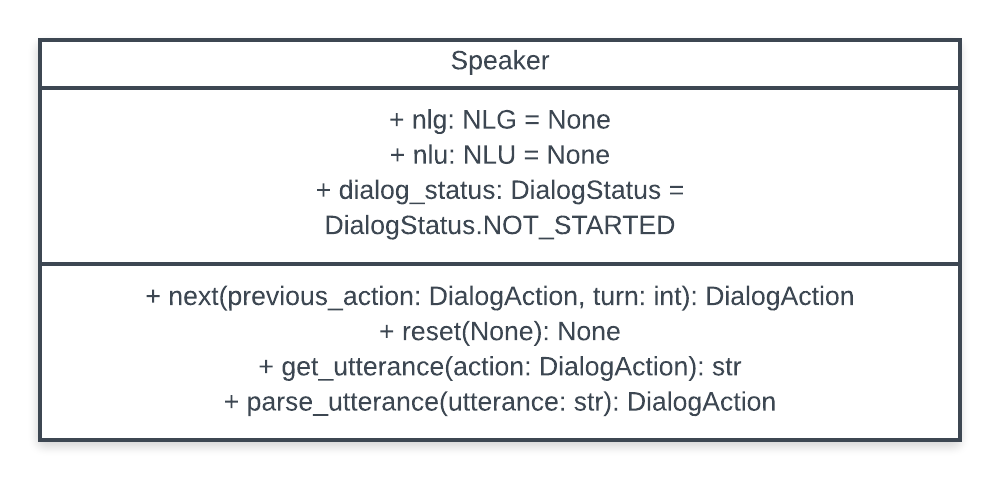
\includegraphics[width=\linewidth]{diagrams/speaker_class.png}
	\caption{ Definition of the Speaker class and methods.}
	\label{fig:speaker_class}
\end{figure}



\subsection{Dialog Domain}

The domain class standardizes the collection and storage of information about the 

\subsubsection{Domain Knowledge Base}


\subsection{Natural Language Understanding}

\subsection{Natural Language Generation}




%%% Local Variables: 
%%% mode: latex
%%% TeX-master: "main"
%%% End: 
